% ============================================================================
%  Refined Index Calculator v0.5 — Workflow diagram (article figure)
%  Envelope: 125 mm (width) x 225 mm (height), portrait.
%  Monochrome (black strokes, white fills); dashed grouping boxes.
% ============================================================================
\documentclass[11pt,border=0pt]{standalone}
\usepackage[T1]{fontenc}
\usepackage{lmodern}
\usepackage{amsmath,amssymb}
\usepackage{tikz}
\usetikzlibrary{arrows.meta,positioning,shapes.geometric,shapes.multipart,%
                fit,backgrounds,calc}

\begin{document}
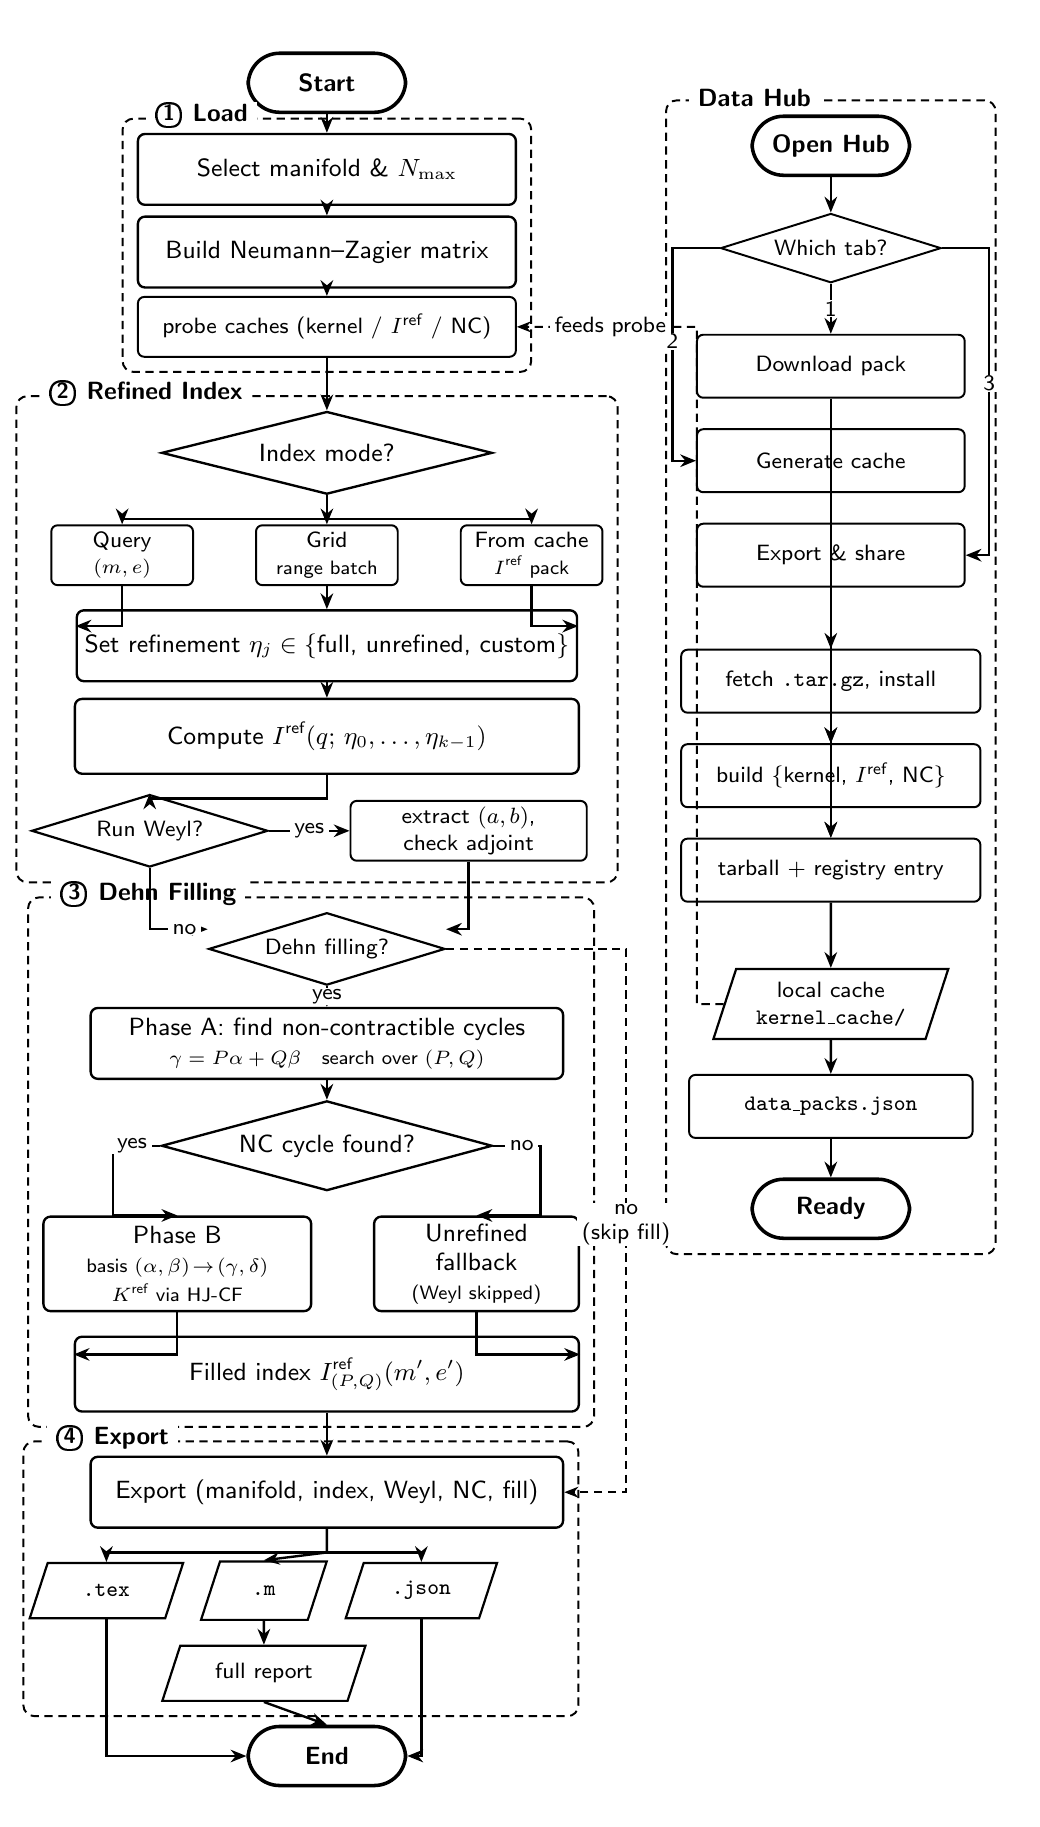
\begin{tikzpicture}[
    x=1mm, y=1mm,
    font=\sffamily\fontsize{9}{10.5}\selectfont,
    %% ── node styles ───────────────────────────────────────────────────────
    M/.style    ={draw=black,line width=0.3mm,fill=white,
                  rounded corners=0.9mm,
                  minimum width=48mm,minimum height=9mm,
                  inner xsep=1mm,inner ysep=0.8mm,align=center},
    Mw/.style   ={M,minimum width=64mm,minimum height=9.5mm},
    Msub/.style ={draw=black,line width=0.25mm,fill=white,
                  rounded corners=0.8mm,
                  minimum width=20mm,minimum height=7.6mm,
                  inner xsep=0.5mm,inner ysep=0.5mm,align=center,
                  font=\sffamily\fontsize{8.2}{9.6}\selectfont},
    Mphase/.style={M,minimum width=30mm,minimum height=12mm},
    Mdec/.style ={draw=black,line width=0.3mm,fill=white,
                  diamond,aspect=2.6,
                  minimum width=42mm,minimum height=10.5mm,
                  inner sep=0mm,align=center,
                  font=\sffamily\fontsize{8.6}{10}\selectfont},
    Msdec/.style={draw=black,line width=0.28mm,fill=white,
                  diamond,aspect=2.4,
                  minimum width=30mm,minimum height=9.2mm,
                  inner sep=0mm,align=center,
                  font=\sffamily\fontsize{8.2}{9.6}\selectfont},
    H/.style    ={draw=black,line width=0.25mm,fill=white,
                  rounded corners=0.8mm,
                  minimum width=34mm,minimum height=8mm,
                  inner xsep=0.6mm,inner ysep=0.4mm,align=center,
                  font=\sffamily\fontsize{8.2}{9.6}\selectfont},
    Hdec/.style ={draw=black,line width=0.25mm,fill=white,
                  diamond,aspect=2.4,
                  minimum width=28mm,minimum height=8.8mm,
                  inner sep=0mm,align=center,
                  font=\sffamily\fontsize{8}{9.4}\selectfont},
    term/.style ={draw=black,line width=0.45mm,fill=white,
                  rounded corners=4mm,
                  minimum width=20mm,minimum height=7.5mm,
                  align=center,
                  font=\sffamily\bfseries\fontsize{9.5}{11}\selectfont},
    data/.style ={draw=black,line width=0.28mm,fill=white,
                  trapezium,trapezium left angle=72,trapezium right angle=108,
                  minimum width=22mm,minimum height=7mm,
                  align=center,
                  font=\sffamily\fontsize{8.2}{9.6}\selectfont},
    stage/.style={draw=black,line width=0.25mm,densely dashed,
                  rounded corners=1.4mm,inner sep=1.8mm},
    stagelbl/.style={font=\sffamily\bfseries\fontsize{9}{10.5}\selectfont,
                  fill=white,inner xsep=1.1mm,inner ysep=0.3mm,
                  anchor=west},
    %% ── arrows ──────────────────────────────────────────────────────────
    ar/.style  ={-{Stealth[length=2mm,width=1.6mm]},line width=0.3mm},
    dar/.style ={-{Stealth[length=1.8mm,width=1.4mm]},line width=0.25mm,
                  densely dashed},
    lbl/.style ={font=\sffamily\fontsize{7.8}{9}\selectfont,
                  inner xsep=0.6mm,inner ysep=0.15mm,fill=white,align=center}
]

\useasboundingbox (0,0) rectangle (125,225);

% =============================================================================
%  Column geometry
%     Main spine x = 38    (calculator pipeline)
%     Hub  spine x = 102   (Data Hub)
%     Right gutter x = 76  (skip arrow) ,  x = 85 (cache cross-link)
% =============================================================================

\node[term] (start) at (38,218) {Start};

% =============================================================================
%  STAGE ① Load
% =============================================================================
\node[M]    (load)  at (38,207)   {Select manifold \& $N_{\max}$};
\node[M]    (nz)    at (38,196.5) {Build Neumann--Zagier matrix};
\node[Msub,minimum width=48mm] (probe) at (38,187)
                                  {probe caches (kernel / $I^{\text{ref}}$ / NC)};

% =============================================================================
%  STAGE ② Refined Index
% =============================================================================
\node[Mdec] (mode)  at (38,171)   {Index mode?};

\node[Msub,minimum width=18mm] (mQ) at (12,158) {Query\\{\scriptsize $(m,e)$}};
\node[Msub,minimum width=18mm] (mG) at (38,158) {Grid\\{\scriptsize range batch}};
\node[Msub,minimum width=18mm] (mC) at (64,158) {From cache\\{\scriptsize $I^{\text{ref}}$ pack}};

\node[M,minimum width=60mm] (eta) at (38,146.5)
   {Set refinement $\eta_j\in\{\text{full, unrefined, custom}\}$};

\node[Mw] (compute) at (38,135)
   {Compute $I^{\text{ref}}(q;\,\eta_0,\ldots,\eta_{k-1})$};

\node[Msdec] (weyl)  at (15.5,123) {Run Weyl?};
\node[Msub,minimum width=30mm] (weylY) at (56,123)
   {extract $(a,b)$,\\check adjoint};

% =============================================================================
%  STAGE ③ Dehn Filling
% =============================================================================
\node[Msdec] (fill)  at (38,108) {Dehn filling?};

\node[M,minimum width=60mm] (findnc) at (38,96)
   {Phase A: find non-contractible cycles\\
    {\scriptsize $\gamma=P\alpha+Q\beta$\ \ \ search over $(P,Q)$}};

\node[Mdec]  (ncfound) at (38,83) {NC cycle found?};

\node[Mphase,minimum width=34mm] (phaseB) at (19,68)
   {Phase B\\{\scriptsize basis $(\alpha,\beta)\!\to\!(\gamma,\delta)$}\\
    {\scriptsize $K^{\text{ref}}$ via HJ-CF}};

\node[Mphase,minimum width=26mm] (unref)  at (57,68)
   {Unrefined\\fallback\\{\scriptsize (Weyl skipped)}};

\node[Mw] (fres) at (38,54)
   {Filled index $I^{\text{ref}}_{(P,Q)}(m',e')$};

% =============================================================================
%  STAGE ④ Export
% =============================================================================
\node[M,minimum width=60mm] (export) at (38,39)
   {Export (manifold, index, Weyl, NC, fill)};

\node[data,minimum width=16mm] (fmtA) at (10, 26.5) {\texttt{.tex}};
\node[data,minimum width=16mm] (fmtB) at (30, 26.5) {\texttt{.m}};
\node[data,minimum width=16mm] (fmtC) at (50, 26.5) {\texttt{.json}};
\node[data,minimum width=24mm] (fmtD) at (30, 16)   {full report};

\node[term] (endnode) at (38,5.5) {End};

% =============================================================================
%  Dashed stage groupings (auto-fit)
% =============================================================================
\begin{scope}[on background layer]
  \node[stage,fit=(load)(nz)(probe)]                              (gLoad) {};
  \node[stage,fit=(mode)(mQ)(mC)(eta)(compute)(weyl)(weylY)]      (gIdx)  {};
  \node[stage,fit=(fill)(findnc)(ncfound)(phaseB)(unref)(fres)]   (gFill) {};
  \node[stage,fit=(export)(fmtA)(fmtC)(fmtD)]                     (gExp)  {};
\end{scope}

\node[stagelbl] at ([xshift=3mm,yshift=0.2mm]gLoad.north west)
   {\textcircled{\footnotesize 1}\,\,Load};
\node[stagelbl] at ([xshift=3mm,yshift=0.2mm]gIdx.north west)
   {\textcircled{\footnotesize 2}\,\,Refined Index};
\node[stagelbl] at ([xshift=3mm,yshift=0.2mm]gFill.north west)
   {\textcircled{\footnotesize 3}\,\,Dehn Filling};
\node[stagelbl] at ([xshift=3mm,yshift=0.2mm]gExp.north west)
   {\textcircled{\footnotesize 4}\,\,Export};

% =============================================================================
%  Main-column arrows  (orthogonal only)
% =============================================================================
\draw[ar] (start)  -- (load);
\draw[ar] (load)   -- (nz);
\draw[ar] (nz)     -- (probe);
\draw[ar] (probe)  -- (mode);

% Mode → 3 sub-modes (T-split bus)
\draw[ar] (mode.south) -- ++(0,-3) -| (mQ.north);
\draw[ar] (mode.south) -- ++(0,-3) -- (mG.north);
\draw[ar] (mode.south) -- ++(0,-3) -| (mC.north);

% 3 sub-modes → eta (merge)
\draw[ar] (mQ.south) |- ([yshift=2.5mm]eta.west);
\draw[ar] (mG.south) -- (eta.north);
\draw[ar] (mC.south) |- ([yshift=2.5mm]eta.east);

\draw[ar] (eta)     -- (compute);

% compute → weyl (left), weyl yes → check (right), both → fill
\draw[ar] (compute.south) -- ++(0,-3) -| (weyl.north);
\draw[ar] (weyl.east)   -- node[lbl,pos=0.5]{yes} (weylY.west);
\draw[ar] (weyl.south)  |- node[lbl,pos=0.8]{no}  ([yshift=2.5mm]fill.west);
\draw[ar] (weylY.south) |- ([yshift=2.5mm]fill.east);

\draw[ar] (fill.south) -- node[lbl,pos=0.5]{yes} (findnc.north);

% fill "no" skip — right gutter at x=76, bypasses stage ③
\draw[dar] (fill.east) -- (76,108) -- (76,39) -- (export.east);
\node[lbl] at (76,73) {no\\{\footnotesize (skip fill)}};

\draw[ar] (findnc)  -- (ncfound);

% NC found? yes → Phase B (left); no → Unrefined (right)
\draw[ar] (ncfound.west) -- ++(-6,0) node[lbl,pos=0.6]{yes} |- (phaseB.north);
\draw[ar] (ncfound.east) -- ++(+6,0) node[lbl,pos=0.6]{no}  |- (unref.north);

% Phase B, Unrefined → Filled index
\draw[ar] (phaseB.south) |- ([yshift=2.5mm]fres.west);
\draw[ar] (unref.south)  |- ([yshift=2.5mm]fres.east);

\draw[ar] (fres)   -- (export);

% Export → 3 formats (T-split) + full report below .m
\draw[ar] (export.south) -- ++(0,-3) -| (fmtA.north);
\draw[ar] (export.south) -- ++(0,-3) -- (fmtB.north);
\draw[ar] (export.south) -- ++(0,-3) -| (fmtC.north);
\draw[ar] (fmtB.south)   -- (fmtD.north);

% Formats → End (merge)
\draw[ar] (fmtA.south) |- (endnode.west);
\draw[ar] (fmtC.south) |- (endnode.east);
\draw[ar] (fmtD.south) -- (endnode.north);

% =============================================================================
%  RIGHT COLUMN — Data Hub
% =============================================================================
\node[term] (hOpen) at (102,210) {Open Hub};
\node[Hdec] (hTab)  at (102,197) {Which tab?};

\node[H]   (hDL)   at (102,182) {Download pack};
\node[H]   (hGN)   at (102,170) {Generate cache};
\node[H]   (hEX)   at (102,158) {Export \& share};

\node[H,minimum width=38mm] (hDLx) at (102,142)
   {fetch \texttt{.tar.gz}, install};
\node[H,minimum width=38mm] (hGNx) at (102,130)
   {build \{kernel, $I^{\text{ref}}$, NC\}};
\node[H,minimum width=38mm] (hEXx) at (102,118)
   {tarball $+$ registry entry};

\node[data,minimum width=30mm] (disk) at (102,101)
   {local cache\\\texttt{kernel\_cache/}};
\node[H,minimum width=36mm]    (reg)  at (102, 88)
   {\texttt{data\_packs.json}};

\node[term] (hReady) at (102, 75) {Ready};

\begin{scope}[on background layer]
  \node[stage,fit=(hOpen)(hTab)(hDL)(hGN)(hEX)(hDLx)(hGNx)(hEXx)(disk)(reg)(hReady)]
       (gHub) {};
\end{scope}
\node[stagelbl] at ([xshift=3mm,yshift=0.2mm]gHub.north west) {Data Hub};

% Data Hub arrows
\draw[ar] (hOpen) -- (hTab);

\draw[ar] (hTab.south) -- node[lbl,pos=0.5]{1} (hDL.north);
\draw[ar] (hTab.west)  -- ++(-6,0) |- node[lbl,pos=0.22]{2} (hGN.west);
\draw[ar] (hTab.east)  -- ++(+6,0) |- node[lbl,pos=0.22]{3} (hEX.east);

\draw[ar] (hDL) -- (hDLx);
\draw[ar] (hGN) -- (hGNx);
\draw[ar] (hEX) -- (hEXx);

\draw[ar] (hDLx) -- (hGNx);
\draw[ar] (hGNx) -- (hEXx);
\draw[ar] (hEXx) -- (disk);
\draw[ar] (disk) -- (reg);
\draw[ar] (reg)  -- (hReady);

% Cross-link: local cache feeds probe caches (dashed, x=85 channel)
\draw[dar] (disk.west) -- (85,101) -- (85,187) -- (probe.east);
\node[lbl] at (74,187) {feeds probe};

\end{tikzpicture}
\end{document}
